
\section{Optimierung des DSP}
In diesem Kapitel soll die Planung und Optimierung des DSP-Codes beschreiben werden.\\
Wie bereits in \textbf{Kapitel \ref{sec:ansatz}} gezeigt wurde, nimmt die Extraktion der zu untersuchenden Features einen Gro�teil der Laufzeit des Programmes ein.
Unter diesem Gesichtspunkt und der in \textbf{Kapitel \ref{sec:davinci}} gezeigten zugrundeliegenden heterogenen Architektur des zu betrachtenden Systems, liegt es nahe, die Extraktion auf dem DSP auszuf�hren.\\
In den nun folgenden Abschnitten sollen daher, wie schon im vorhergehenden Kapitel erst die Bottlenecks identifiziert (\textbf{\ref{sec:ansatzdsp}}) und danach die durchgef�hrten Optimierungen beschrieben werden (\textbf{\ref{sec:mathlib}} - \textbf{\ref{sec:compiler}}).

\subsection{Bottlenecks des DSP-Codes}\label{sec:ansatzdsp}

F�r die Laufzeitmessungen des DSP-Codes wurden wie schon im vorherigen Kapitel die FeaturesSets 1-4 (\textbf{\ref{subsec:fset1}} - \textbf{\ref{subsec:fset4}}) verwendet.
Die ben�tigen Zeiten wurden auch hier wieder mit der Gesamtzeit in Verh�ltnis gesetzt, wodurch die aus \textbf{Abbildung \ref{fig:dsp}} zu entnehmenden Anteile der einzelnen Features an der Gesamtlaufzeit errechnet wurden.\\
%
\begin{figure}
	\centering
		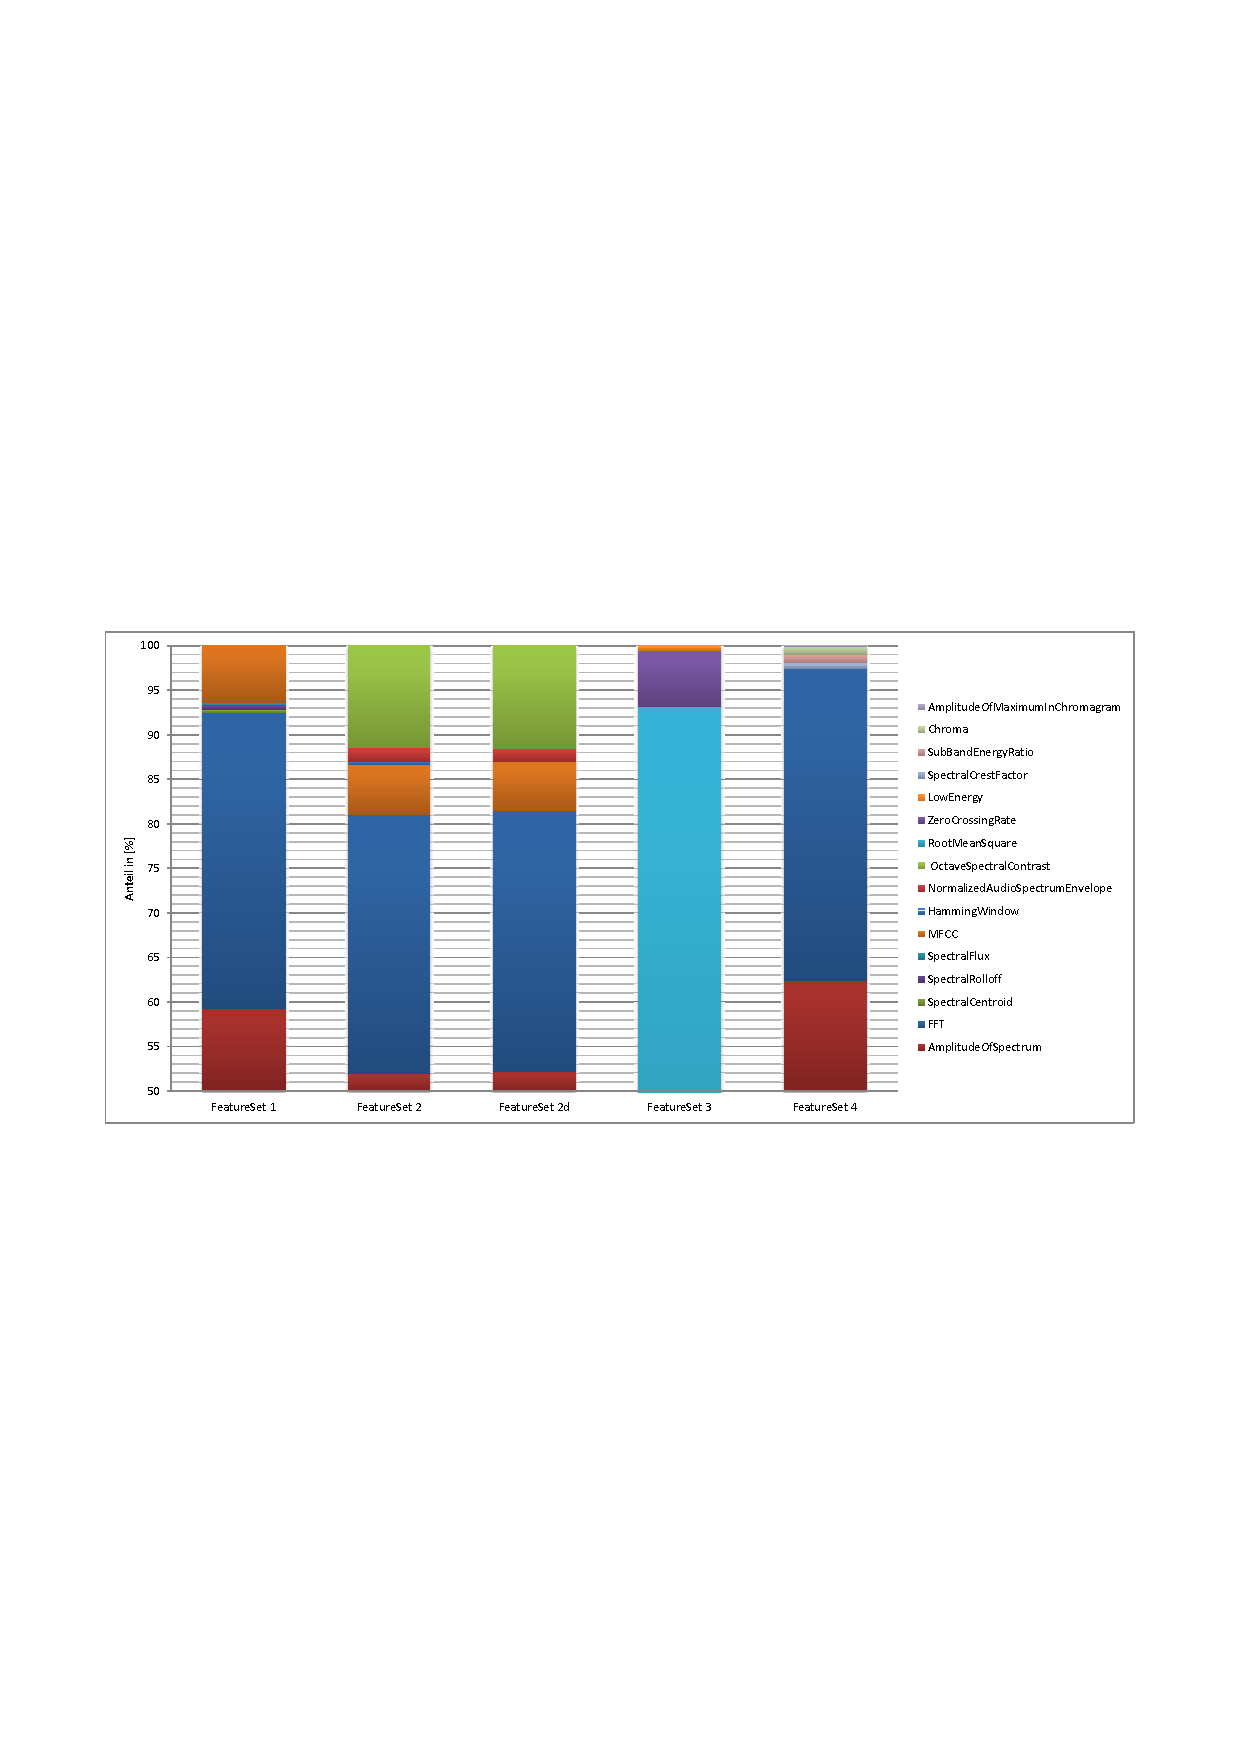
\includegraphics[width=1.00\textwidth]{../Pictures/ResultsExtraktionDSP.pdf}
	\caption{Laufzeitanteile der Features auf dem DSP}
	\label{fig:dsp}
\end{figure}
%
Es ist deutlich zu erkennen, dass in den FeatureSets 1 - 2d und 4 \textit{Amplitude of Spectrum} (\textbf{\ref{subsubsec:aos}}) und im FeatureSet 3 \textit{Root Mean Square} (\textbf{\ref{subsubsec:rms}}) die meiste Laufzeit in Anspruch nehmen, teilweise mit Anteilen weit �ber 50\%. Da beide Features eigentlich nur aus Summationen, Divisionen und der Bildung von Quadratwurzeln bestehen, die Bestandteil der Standartbibliotheken sind, scheint bei der Ausf�hrung von mathematischen Funktionen ein Bottleneck zu entstehen. Des weiteren ist zu sehen, dass auch bei der Umsetzung des Codes auf dem DSP ein weiterer Bottleneck bei der Ausf�hrung der FFT zu bestehen scheint, da auch diese mit ca. 30\% der Ausf�hrungszeit zu Buche schl�gt.

\subsection{Optimierung der Rechenfunktionen mit MATHLIB}\label{sec:mathlib}
MATHLIB ist eine von Texas Instruments mit dem EZSDK mitgelieferte Bibliothek von Mathematikfunktionen, die f�r die Benutzung auf dem C674x optimiert sind. Insbesondere bietet diese Bibliothek optimierte Berechnungen von Wurzel-, Quadrierungs- und Divisionsfunktionen, welche in fast jedem in \textbf{Kapitel \ref{sec:alg}} vorgestellten Algorithmen verwendet werden.\\
Die einzelnen Ausf�hrungszeiten eines Aufrufes eines dieser Funktionen f�llt nicht unbedingt als Bottleneck auf, da diese aber in den meisten Algorithmen f�r jedes Fenster und dann h�ufig auch innerhalb von Schleifen ausgef�hrt werden, summiert sich ihre Ausf�hrungszeit stark auf.\\
Die von der Bibliothek MATHLIB angebotenen Funktionen boten sich hier besonders deswegen an, dass sie nicht nur die M�glichkeit bieten einzelne Aufrufe durch MATHLIB-Aufrufe zu ersetzen, sondern diese auch die Option bietet, ganze Vektoren einer zum Beispiel Wurzelfunktion zuzuf�hren und somit die Parallelit�t des C674x zu unterst�tzen.\\
Zu erw�hnen ist dabei allerdings, dass die von MATHLIB zur Verf�gung gestellten "`Vektoroperationen"' nur auf Vektoren des Typs Double funktionieren, die zu berechnenden Werte jedoch im Floatformat vorliegen. Daraus ergibt sich, dass zur Vorbereitung f�r solche Funktionen die Floatvektoren erst in Doublevektoren umgewandelt werden mussen, was erstens weitere Schleifen vor und nach den Algorithmen zur Folge hat und zweitens durch die Allokation von Doublearrays auch einen erh�ten Speicherbedarf zur Folge hat. Da in dieser Arbeit aber einzig auf die Ausf�hrungszeit hin optimiert werden sollte, ist der zweite Einwand zu vernachl�ssigen.\\
Beispielhaft kann die Code�nderung am Beispiel von \textit{Amplitude of Spectrum} (\textbf{\ref{subsubsec:aos}}) in \textbf{Listing \ref{code:aos}} und \textbf{Listing \ref{code:aoso}} entnommen werden.

\begin{lstlisting}[caption=Urspr�nglicher Amplitude of Spectrum Code, label=code:aos]

for (k = 0; k < G; ++k) {
	A[k] = sqrt(X[k] * X[k] + Y[k] * Y[k]) / G;
}

\end{lstlisting}

\begin{lstlisting}[caption=Optimierter Amplitude of Spectrum Code, label=code:aoso]
realv tmp1;
realv tmp2;

atemp = (double*) malloc(G * sizeof(double));
pG = (double*) malloc(G * sizeof(double));
divtemp = (double*) malloc(G * sizeof(double));
int f;
for (f = 0; f < G; ++f) {
	pG[f] = (double) G;
}

for (k = 0; k < G; ++k) {
	tmp1 = X[k] * X[k];
	tmp2 = Y[k] * Y[k];
	atemp[k] = (double) (tmp1 + tmp2); //(X[k] * X[k] + Y[k] * Y[k]);
		}

sqrtdp_v(atemp, atemp, G);

divdp_v(atemp, pG, divtemp, G);

for (k = 0; k < G; ++k) {
	A[k] = (float) divtemp[k];

}

\end{lstlisting}

 

\subsection{Optimierung der FFT mit DSPLIB}\label{sec:dsplib}

\subsection{Optimierung f�r den Compiler}\label{sec:compiler} 